\documentclass[11pt,a4paper]{article}
\newcommand{\ReportFooter}{Seolwongyeong multiplayer server}
\usepackage[margin=20mm, top=19mm, bottom=20mm]{geometry}
\usepackage{fontspec}
\setmainfont{texgyrepagella}[
  Extension=.otf, UprightFont=*-regular, ItalicFont=*-italic,
  BoldFont=*-bold, BoldItalicFont=*-bolditalic]
\setsansfont{texgyreheros}[
  Extension=.otf, UprightFont=*-regular, ItalicFont=*-italic,
  BoldFont=*-bold, BoldItalicFont=*-bolditalic]
\usepackage{amsmath}
\usepackage{graphicx}
\graphicspath{{../images/}}
\usepackage{booktabs, tabularx}
\usepackage{caption}
\usepackage{enumitem}
\usepackage{placeins}
\usepackage{titlesec}
\usepackage{fancyhdr}
\usepackage{cite}
\usepackage{xcolor}
\usepackage{xurl}
\usepackage[unicode]{hyperref}

\definecolor{accent}{HTML}{204E77}
\definecolor{muted}{HTML}{455464}
\definecolor{rulegray}{HTML}{CAD3DC}
\hypersetup{colorlinks=true, linkcolor=accent, citecolor=accent, urlcolor=accent}
\urlstyle{same}

\setlength{\parindent}{0pt}
\setlength{\parskip}{5.5pt plus 1pt}
\linespread{1.05}
\raggedbottom
\clubpenalty=10000
\widowpenalty=10000
\setlist{topsep=2pt, itemsep=2pt, parsep=0pt, leftmargin=1.65em}
\setlength{\textfloatsep}{14pt plus 2pt minus 3pt}
\setlength{\intextsep}{12pt plus 2pt minus 2pt}
\setlength{\tabcolsep}{5pt}
\renewcommand{\arraystretch}{1.25}
\newcolumntype{L}{>{\raggedright\arraybackslash}X}
\newcolumntype{P}[1]{>{\raggedright\arraybackslash}p{#1}}
\captionsetup{font=small, labelfont=bf, labelsep=period, justification=raggedright,
  singlelinecheck=false, skip=7pt}
\AddToHook{env/thebibliography/begin}{\small\raggedright}

\titleformat{\section}{\Large\sffamily\bfseries\color{accent}}{\thesection}{0.65em}{}
\titleformat{\subsection}{\large\sffamily\bfseries}{\thesubsection}{0.65em}{}
\titlespacing*{\section}{0pt}{15pt plus 2pt minus 2pt}{5pt}
\titlespacing*{\subsection}{0pt}{11pt plus 2pt minus 2pt}{3pt}

\pagestyle{fancy}
\fancyhf{}
\renewcommand{\headrulewidth}{0pt}
\renewcommand{\footrulewidth}{0.3pt}
\fancyfoot[L]{\sffamily\small\color{muted}\ReportFooter}
\fancyfoot[R]{\sffamily\small\color{muted}\thepage}

\newcommand{\ReportTitle}[3]{%
  {\sffamily\bfseries\small\color{accent}#1\par}
  \vspace{5pt}
  {\sffamily\bfseries\fontsize{22}{27}\selectfont\raggedright #2\par}
  \vspace{4pt}
  {\sffamily\small\color{muted}#3\par}
  \vspace{2pt}
  {\color{rulegray}\hrule}
}

\newcommand{\code}[1]{\texttt{#1}}
\newcommand{\change}[2]{#1 \(\to\) #2}

\newcommand{\ReportFigure}[3]{%
  \par\medskip
  \noindent\begin{minipage}{\linewidth}
    \captionsetup{type=figure}
    \includegraphics[width=\linewidth]{#1}\par
    \caption{#2}
    \label{#3}
  \end{minipage}\par
}

\newcommand{\DeltaRows}{%
   50 & \change{62.5}{27.6} & \change{3.05}{1.35} \\
  100 & \change{65.3}{28.9} & \change{6.38}{2.82} \\
  200 & \change{70.8}{28.4} & \change{13.83}{5.54} \\
  400 & \change{54.5}{23.4} & \change{21.30}{9.14} \\
}

\newcommand{\UbuntuRows}{%
    400 &  47\% & 14.5 & 40 / 74 \\
    800 & 100\% & 13.6 & 49 / 91 \\
  1,000 & 133\% & 11.8 & 55 / 103 \\
  1,200 & 125\% &  7.8 & 161 / 237 \\
}

\newcommand{\StageRows}{%
  100 & 14.5 / 71  & 15.0 / 71  & \change{19\%}{11\%} \\
  200 & 14.0 / 77  & 15.0 / 74  & \change{37\%}{19\%} \\
  400 & 10.8 / 296 & 15.0 / 78  & \change{63\%}{33\%} \\
  800 &  8.0 / 725 & 15.0 / 325 & \change{71\%}{48\%} \\
}

\newcommand{\ProductionRows}{%
    200 & 15.0 & 39 / 75          & 71\%          & 30\%         & 26\% \\
    400 & 15.0 & 49 / 85          & 113\%         & 58\%         & 47\% \\
    600 & 15.0 & 52--53 / 95--98  & 158--161\%    & 87--90\%     & 63--65\% \\
    700 & 15.0 & 57 / 114         & 180\%         & 101\%        & 73\% \\
    800 & 15.0 & 75--101 / 163--275 & 189--197\%  & 90--108\%    & 87--94\% \\
  1,000 & 12.7 & 237 / 3,467      & 197\%         & 100\%        & 91\% \\
  1,200 & 14.3 & 445 / 1,309      & 200\%         & 92\%         & 91\% \\
}

\hypersetup{
  pdftitle={Performance Optimization and Load Testing of the Seolwongyeong Multiplayer Server},
  pdflang={en}
}

\begin{document}
\ReportTitle{Research report}
  {Performance Optimization and Load Testing of the Seolwongyeong Multiplayer Server}
  {Production load test \enspace\textbar\enspace November 14, 2026}

\pdfbookmark[1]{Abstract}{abstract}
\section*{Abstract}
This report presents a load test of the multiplayer server for Seolwongyeong
(\href{https://ski.stelide.com}{ski.stelide.com}), a Korean-language metaverse ski resort.
We increased concurrency in stages on a two-core Oracle Ampere production server and measured
position delivery latency, update rate, network traffic, and per-process CPU usage. We estimated
that the Python implementation could serve about 450 concurrent players smoothly. We introduced
delta encoding for changed fields, fixed file descriptor exhaustion caused by leaked database
connections, raised the connection limit from 400 to 2,000, and reimplemented the real-time relay
in Go. At 700 concurrent players, p99 position delivery latency was 114\,ms and the server sustained
15 updates per second. CPU usage approached saturation at 800 players, and p99 latency rose into the
seconds at 1,000 and above. The highest tested load that met the smoothness criteria was 700
players on the test path, which excluded TLS. The case demonstrates how interest management
and incremental state transmission can help a small commercial service under measured load.

{\small\textbf{Keywords} \quad Metaverse server, performance optimization, load testing,
interest management, incremental state transmission.}

\section{Introduction}
Seolwongyeong is a metaverse ski resort where players exchange avatar positions in real time.
Relaying those positions consumes CPU and bandwidth as concurrency grows and is the first component
to saturate. This report measures the production server's capacity, identifies and addresses the
bottlenecks, and quantifies the remaining limits and options for further improvement.

The study makes four contributions. First, we built a load-testing harness that reproduces the
game engine's movement and identified and corrected distortions due to harness scheduling aligning
with server ticks and due to same-host measurement. Second, sending only changed fields cut
per-player inbound traffic by 56--60\%. Third, we diagnosed and fixed two resource limits, a file
descriptor leak and connection caps. Fourth, we measured the scalability ceiling imposed by
Python's global interpreter lock (GIL) and moved the real-time relay to Go. On STAGE, the Go relay
used about \(1/2.2\) as much CPU per player as the Python relay. Measured smooth capacity with Go
was about 1.5 times the earlier Python estimate.

\section{Related work}
Server scalability is a longstanding problem in multiplayer online games. In client-server
architectures, central server bandwidth requirements can grow faster than the player count.
Pellegrino and Dovrolis identified this bottleneck by examining the trade-off between server
bandwidth and the cost of maintaining state consistency among peers~\cite{pellegrino_2003_12}.
Kim proposed a hybrid server-peer design to reduce that bandwidth requirement~\cite{kim_2013}.

Interest management is a standard way to limit traffic. Broadcasting every state change to every
participant in a large distributed simulation rapidly increases the number of deliveries. Early
work organized techniques that forward only relevant updates~\cite{morse_2000_1}, and a later
survey classified design choices and their trade-offs~\cite{liu_2014_2}. Measurements in an
actual game found that obstacle-aware interest management could cut the update count by a factor
of up to six. A less expensive tile-based algorithm approximated the ideal visibility-based
scheme~\cite{boulanger_2006_10}. Cloud deployments have used publish/subscribe interest sets to
reduce bandwidth and scale to hundreds of players~\cite{najaran_2010_5}. Adaptive pub/sub
middleware has also been proposed to filter state updates against a bandwidth
budget~\cite{gascon_samson_2015_6}.

The simplest incremental state representation in this report sends only changed fields.
Orsten used prediction, learning, and entropy coding to synchronize hundreds of entities with
less than a few kilobytes per second~\cite{orsten_2011_4}. Work on dynamic web content likewise
used temporal correlation in delta encoding to reduce bandwidth~\cite{psounis_2002_11}. Prior
work commonly evaluates large multiplayer games or simulations in simulations and testbeds.
This case measures a small commercial service on its production infrastructure, including nginx
and kernel networking, and quantifies the CPU impact of the GIL and the reverse proxy.

\section{System architecture}
The Go relay batches position updates by room and sends the same frame to every player in that
room 15 times per second (15\,Hz). The Python server handles pages, login, rankings, and database
operations. A slope-channel room normally accommodates 40 players, with a server-side cap of
48. Parties use separate rooms. Figure~\ref{fig:architecture} shows the player-facing traffic path.

On joining, a client receives a full state snapshot (\code{u}). Subsequent frames carry changed
fields (\code{v}), and a departure is signaled with \code{x}. Each \(1/15\)-second tick batches
the players whose positions changed. The relay suppresses implausibly abrupt position changes.
The server is authoritative for collisions and checks speed and distance when resolving them.
The server caps total concurrent connections at 2,000 and enforces per-IP connection limits and
per-connection message rates. The previous Python relay remains available through a one-line
nginx configuration change.

\begin{figure}[!htbp]
  \centering
  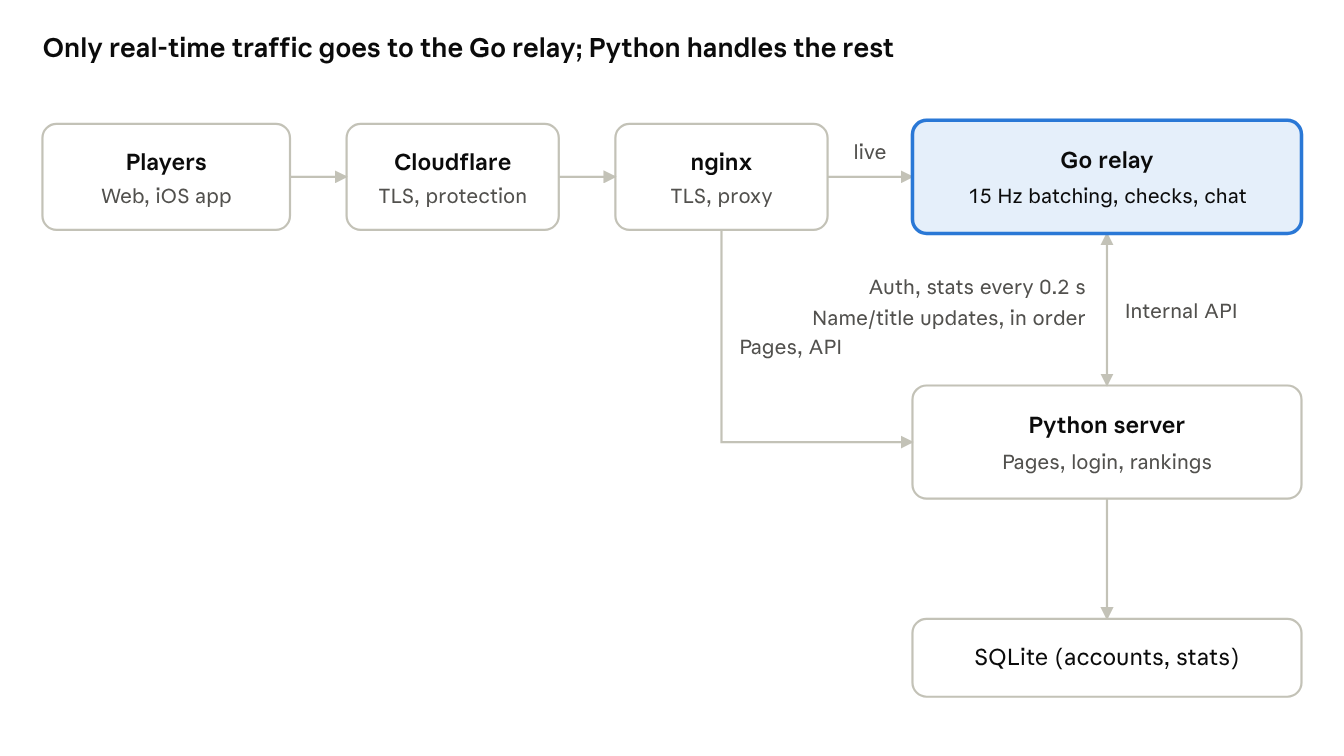
\includegraphics[width=\linewidth]{architecture.en.png}
  \caption{Player-facing architecture. nginx routes live traffic to the Go relay and pages and
    API calls to Python. Python handles SQLite access. The production load tests used the
    direct HTTP test path described in Section~\ref{sec:limits}.}
  \label{fig:architecture}
\end{figure}
\FloatBarrier

\section{Measurement method}
We tested with a harness that connects simulated players to the server. We first wrote the
harness in Python (\code{server/bench\_net.py}), then rewrote it in Go to generate higher
production loads. Simulated players follow the game engine's sequence. They select a ski area in
the lobby, join a 40-player slope-channel room, and send positions 15 times per second. Positions
follow wall-clock time, and reported speeds match those movements so the server accepts them as
plausible. Each player sends at fixed intervals (\(t_0 + k/15\) seconds), with a different phase
offset for each player.

\begin{itemize}
  \item \textbf{Latency.} One probe in each room measures the time for a position sent by
    another player to reach it. The sender and probe run in the same process, so they share a
    clock. The measurement includes the wait for the next 15\,Hz frame, which averages 33\,ms.
  \item \textbf{Update rate.} Room updates received per second by the probe. The target is 15.
  \item \textbf{Traffic.} Bytes sent and received per connection, including WebSocket frame
    headers. TCP/IP headers are excluded.
  \item \textbf{Server CPU.} Usage for the Go relay, Python, and nginx measured separately
    through \code{/proc}, plus total CPU on production. One fully utilized core counts as 100\%.
  \item \textbf{Stability.} Counts of dropped connections and rejected room joins.
\end{itemize}

Table~\ref{tab:environments} lists the three test environments. Each load level had an
8-second warm-up and a 30-second measurement window. We recorded one run at most levels.
The 600- and 800-player production levels were run twice and are reported as ranges
(Section~\ref{sec:limits}). For the production test, we opened a temporary route restricted to the
two load generators and closed it afterward. Bots joined channels unused by real players.

\begin{table}[!htbp]
  \caption{Test environments. Dates are in November 2026.}
  \label{tab:environments}
  \small
  \begin{tabularx}{\linewidth}{@{}P{0.22\linewidth}P{0.18\linewidth}L P{0.21\linewidth}@{}}
    \toprule
    \textbf{Environment} & \textbf{CPU} & \textbf{Server and harness placement} & \textbf{Purpose} \\
    \midrule
    Production (Nov. 14) & Ampere, 2 cores & Two remote hosts (STAGE and bot server), over the network via nginx & Measure production capacity \\
    Ubuntu i5-11600K (Nov. 11) & Server pinned to 2 cores & Same host, separate cores & Assess Python capacity \\
    STAGE (Nov. 11) & Ampere, 1 core & Server and harness share one core & Compare implementations \\
    \bottomrule
  \end{tabularx}
\end{table}
\FloatBarrier

\section{Optimization}
The main bottleneck shifted from bandwidth to file descriptors, then to Python's GIL, and
finally to nginx and kernel networking.

\subsection{Delta encoding for changed fields}
The previous implementation sent the full position state on every update. We changed it to send
a full state (\code{u}) once and then only changed fields (\code{v}).
Table~\ref{tab:delta} compares the two encodings on the same single-core STAGE environment.

\begin{table}[!htbp]
  \caption{Traffic before and after delta encoding on STAGE.}
  \label{tab:delta}
  \small
  \begin{tabular*}{\linewidth}{@{\extracolsep{\fill}}rrr@{}}
    \toprule
    \textbf{Concurrent connections} & \textbf{Inbound per player (KB/s)} & \textbf{Server outbound (MB/s)} \\
    \midrule
    \DeltaRows
    \bottomrule
  \end{tabular*}
\end{table}

Inbound traffic per player and server outbound traffic fell by 56--60\%. CPU usage changed little
because the server still assembled and validated frames. This result is consistent with the
traffic reductions reported for interest management~\cite{boulanger_2006_10} and incremental
state transmission~\cite{orsten_2011_4}.

\subsection{File descriptor leak}
At about 330 concurrent connections, \code{/ws} returned HTTP 500 errors. The connection handler
did not return until the connection closed, leaving a SQLite connection open. Each client
connection consumed three file descriptors, exhausting the default limit of 1,024. Closing the
database connection immediately left one socket per client connection. At 100 players, the total
descriptor count fell from 305 to 104. The connection errors near 330 players did not recur
after the fix.

\subsection{Higher connection limits}
We raised the server-wide cap from 400 to 2,000 connections, nginx
\code{worker\_connections} to 8,192, and the systemd service setting \code{LimitNOFILE} to 65,536.
CPU then became the limiting resource.

\subsection{Python's GIL and the Go relay}
With the Python server pinned to two cores on the Ubuntu test machine, CPU usage plateaued at
125--133\% (Table~\ref{tab:ubuntu}). The GIL allowed only one thread at a time to execute Python
code, so adding a second core yielded a gain of about 25\%.

\begin{table}[!htbp]
  \caption{Two-core Python server on Ubuntu.}
  \label{tab:ubuntu}
  \small
  \begin{tabular*}{\linewidth}{@{\extracolsep{\fill}}rrrr@{}}
    \toprule
    \textbf{Concurrent connections} & \textbf{CPU (max. 200\%)} & \textbf{Updates/s} & \textbf{p50 / p99 (ms)} \\
    \midrule
    \UbuntuRows
    \bottomrule
  \end{tabular*}
\end{table}

Allowing for the roughly 1.75-fold per-core speed difference between the Ubuntu machine and
the production server, we estimated that the production Python server would run smoothly up to
about 450 players and reach its limit near 570. We moved room management, position frame assembly,
relay validation, chat, and parties to Go. Pages, login, rankings, and database operations stayed
in Python. Table~\ref{tab:stage} compares the two implementations on the same STAGE core.

\begin{table}[!htbp]
  \caption{Python and Go on one STAGE core. Each relay column shows updates/s and p99 latency in ms.}
  \label{tab:stage}
  \small
  \begin{tabular*}{\linewidth}{@{\extracolsep{\fill}}rrrr@{}}
    \toprule
    \textbf{Concurrent connections} & \textbf{Python} & \textbf{Go} & \textbf{CPU (Python to Go)} \\
    \midrule
    \StageRows
    \bottomrule
  \end{tabular*}
\end{table}

CPU usage per player was 0.185\% for Python and 0.083\% for Go, a ratio of about 2.2.
At 800 players, sharing a STAGE core with the harness increased Go latency.
The Go relay entered production on November 12, 2026.
\FloatBarrier

\section{Production results}
\label{sec:results}
We define smooth operation as maintaining 15 updates per second with p99 position delivery
latency at or below 150\,ms. The cutoff is informed by a reference game experiment in which
end-to-end delay below 150\,ms was hard to perceive~\cite{nister_compact_game_data}, and the
observation that \emph{Quake 3} players tended to prefer servers below 150--180\,ms of
ping~\cite{armitage_2003_9}. Tolerance varies by genre and interaction~\cite{raaen_2014_3}.
Here, 150\,ms is the criterion applied to the harness's position delivery metric.

On November 14, 700 concurrent players met both criteria with p99 at 114\,ms and 15.0 updates
per second. At 800, total CPU reached 189--197\% of a 200\% maximum, and p99 rose to 163--275\,ms.
From 1,000 players, p99 was measured in seconds. Table~\ref{tab:production} gives the readings
at each load, and Figure~\ref{fig:capacity} shows the latency and CPU trends.

\begin{table}[!htbp]
  \caption{Production load test on November 14, 2026. Ranges show the two readings at 600 and 800 connections.}
  \label{tab:production}
  \small
  \begin{tabular*}{\linewidth}{@{\extracolsep{\fill}}rrrrrr@{}}
    \toprule
    \textbf{Connections} & \textbf{Updates/s} & \textbf{p50 / p99 (ms)} &
    \shortstack[r]{\textbf{Total CPU}\\(max. 200\%)} & \textbf{Go relay} & \textbf{nginx} \\
    \midrule
    \ProductionRows
    \bottomrule
  \end{tabular*}
\end{table}

No connections dropped and no room joins were rejected at any load level. As the server became
saturated, it kept connections open and delivered updates later. Per-player inbound traffic was
13--21\% lower at 800 connections and nearly halved at 1,000 or more.

CPU usage per player was about 0.14\% for the Go relay and 0.10\% for nginx. In these estimates,
nginx used about 70\% as much CPU as the relay.\footnote{The Korean PDF supplied as the source
described nginx usage as 70\% higher. The per-player estimates and the readings at 700
connections (73\% for nginx and 101\% for Go) support the corrected ratio.}
Most remaining CPU usage was attributed to kernel network processing. The Python server used
0--1\% because the bots joined as guests and did not require login checks or forward game records.
CPU usage on the two load generators remained at 66--72\% at 1,200 players, indicating that the
server constrained capacity.

The smooth capacity with Go was about 1.5 times the earlier Python estimate of 450 players.
The comparison uses a measured result and an estimated baseline. The relay became about 2.2
times as CPU-efficient on STAGE, and the unchanged costs of nginx and kernel networking limited
the gain in overall capacity.

\ReportFigure{prod-capacity.en.png}
  {Position delivery latency (top, logarithmic scale) and CPU usage (bottom).
    The dashed line marks the highest tested load that met the smoothness criteria.
    CPU bars at 600 and 800 connections average two runs.}
  {fig:capacity}

\section{Discussion}
\textbf{Changing bottlenecks and remaining costs.}
Each optimization exposed the next constraint, from bandwidth and descriptors to the GIL and
then nginx and kernel networking. Once the relay was more efficient, the reverse proxy and kernel
accounted for a substantial share of the remaining cost. An implementation language change alone
can therefore deliver a smaller system-level gain than its effect on the component it replaces.

\textbf{Measurement pitfalls.}
Three features of the test setup affected the results. First, the early harness slept \(1/15\)
second after each send, causing bots to send in a burst just after a server tick and inflating
latency to 61\,ms. Fixed intervals with per-player phase offsets corrected this. Real players on
separate devices do not synchronize in this way. Second, on a shared single core, the harness
used more CPU than the Go relay. The Python harness reached about 300 players on one core, and
the Go production harness generated about 650. Third, same-host tests yielded lower CPU costs
than the networked production path. The Go relay used 0.083\% per player on STAGE and 0.14\% in
production. We used same-host measurements to compare implementations and used networked
production measurements to establish capacity. We computed per-player costs from loads of
200 or more to reduce the influence of fixed overhead. These precautions are consistent with
conditions under which bot-based tests can approximate live measurements~\cite{boulanger_2006_10}.

\textbf{Relation to earlier work.}
Visibility- and obstacle-based filtering can substantially reduce message counts~\cite{boulanger_2006_10}.
In Seolwongyeong, coarse spatial partitioning by room was sufficient. Visibility occlusion has
little effect on skiing gameplay, and broadcasting to a 40-player room is likely cheaper than
computing which updates each player should receive. The decrease from 15.0 to 12.7 updates per
second and the lower inbound traffic in Section~\ref{sec:results} suggest that saturation led
to effective backpressure through delayed delivery. This differs in mechanism from adaptive
filtering that deliberately enforces a bandwidth budget~\cite{gascon_samson_2015_6}.
\section{Limitations}
\label{sec:limits}
\begin{itemize}
  \item \textbf{Server-side test path.} The production test reached nginx over plain HTTP.
    Players normally connect through Cloudflare and TLS. That additional work could lower the
    capacity on the live path.
  \item \textbf{Heavier simulated workload.} Bots were continuously active in full 40-player
    rooms. Actual players stop sending positions in menus and on the lift pass screen, and
    rooms can be partially occupied. These differences make the simulated movement load
    conservative.
  \item \textbf{Limited replication.} We ran most load levels once. The p99 measurements of
    163 and 275\,ms at 800 players illustrate the variability near saturation.
  \item \textbf{Validation scope.} We checked collision detection with server unit tests.
    We checked position delivery, chat, and parties in the actual game interface.
\end{itemize}

\section{Conclusion and future work}
Actual concurrency at the time of the report was in the single digits, leaving ample headroom
relative to the tested capacity. The following changes are priorities if traffic grows.

\begin{enumerate}
  \item \textbf{Route live traffic directly to Go.}
    Use Cloudflare Origin Rules to route only \code{/ws} to the Go relay on a separate port,
    with Go terminating TLS. Player URLs and the iOS app can stay as they are. Recovering the
    roughly 40\% of total CPU used by nginx at 700 players could raise capacity to 900--1,000
    players. Go would need to enforce per-IP connection rate limits, reject slow connections,
    identify the real client IP via \code{CF-Connecting-IP}, and manage certificates. The
    availability of the required Origin Rules on the free plan remains to be verified.
  \item \textbf{Send fewer bytes.}
    Reducing numeric precision could cut traffic by 20--30\% with a small change. Lowering
    the update rate from 15 to 10\,Hz would cut updates and bytes by one third, subject to
    checking the effect on visual smoothness. Varying the update rate by distance could save
    50--70\% of bytes. Since it requires recipient-specific frames, its CPU impact needs to be
    measured. Any approach must remain compatible with the deployed iOS app and bot server.
  \item \textbf{Add CPU cores.}
    Upgrade the production server to a paid configuration with more cores as a last resort.
\end{enumerate}

Table~\ref{tab:alternatives} summarizes the alternatives considered during the review.

\begin{table}[!htbp]
  \caption{Alternatives considered and reasons for rejecting them.}
  \label{tab:alternatives}
  \small
  \begin{tabularx}{\linewidth}{@{}P{0.33\linewidth}L@{}}
    \toprule
    \textbf{Alternative} & \textbf{Reason} \\
    \midrule
    Rewrite the whole server in Go & The real-time relay was the bottleneck. Pages and APIs had little load. \\
    Move the relay to single-core STAGE & Estimated smooth capacity would fall to 450--550 players and the test server would be lost. \\
    Spread the relay across three servers & The cost of keeping lobby, party, and chat state consistent would outweigh the benefits. \\
    WebSocket compression (\code{permessage-deflate}) & Compression saves bandwidth but adds CPU work to a CPU-bound server. \\
    \bottomrule
  \end{tabularx}
\end{table}

The remaining measurements are capacity on the player-facing path with TLS and a new test after
routing live traffic directly to Go. This report is released under
\href{https://creativecommons.org/licenses/by/4.0/}{CC BY 4.0}. The
\href{https://github.com/somany-flower4u/multiplayer-perf-report}{project repository} contains
both language editions and the source figures.
\FloatBarrier

\bibliographystyle{IEEEtran}
\bibliography{references}
\end{document}
